% !TeX spellcheck = en_EN
% !TeX encoding = UTF-8
% !TeX program = xelatex
% !BIB program = bibtex
\documentclass[english,10pt,xcolor=colortbl,compress]{beamer}
\usepackage{xunicode}
\usepackage[T1]{fontenc}
\usepackage{calc}
\usepackage[ngerman]{babel} % Neue Rechtschreibung
\usepackage{amsmath,amsthm,amssymb,euscript} % AMS-LaTeX  
\usepackage{enumerate,graphicx}
\usepackage{forest} 
\usepackage{graphicx} 
\usepackage{booktabs} 
\usepackage{listings}
\usepackage{tikz}
\usepackage[export]{adjustbox}
\usepackage{multirow}
\usepackage{algorithm, algpseudocode}
\usetheme[
slogan=false, 
navigation=true,
frametotal,
myriad=true,
footline=true,
ITMtheme
]{UZL}
\setbeamertemplate{navigation symbols}{}
\usetikzlibrary{positioning,matrix,shapes.arrows,calc,snakes}
\title[]{Simulation Framework for Distributed Database Query Processing in
the Semantic Internet of Things}
\author[Johann Mantler]{Johann Mantler}

\institute[Master’s Thesis] 
{   Master’s Thesis \\
    Institute of Information Systems \\
	University of Lübeck \\
	\medskip
	\textit{supervised by} \\
	Prof. Dr. Sven Groppe, \\
	Benjamin Warnke
}
\date{12. August 2021} 
\newcommand\blfootnote[1]{%
	\begingroup
	\renewcommand\thefootnote{}\footnote{#1}%
	\addtocounter{footnote}{-1}%
	\endgroup
}
\addtobeamertemplate{frametitle}{\vspace*{-1.0ex}}{\vspace*{-6.0ex}}


\begin{document}
\newcommand{\RNum}[1]{\uppercase\expandafter{\romannumeral #1\relax}}	
	
	
\begin{frame}

	\titlepage 
\end{frame}


\section{Introduction}
% \begin{frame}
% 	\frametitle{Increasing Number of IoT Devices}
% 	\begin{figure}
% 		\centering
% 		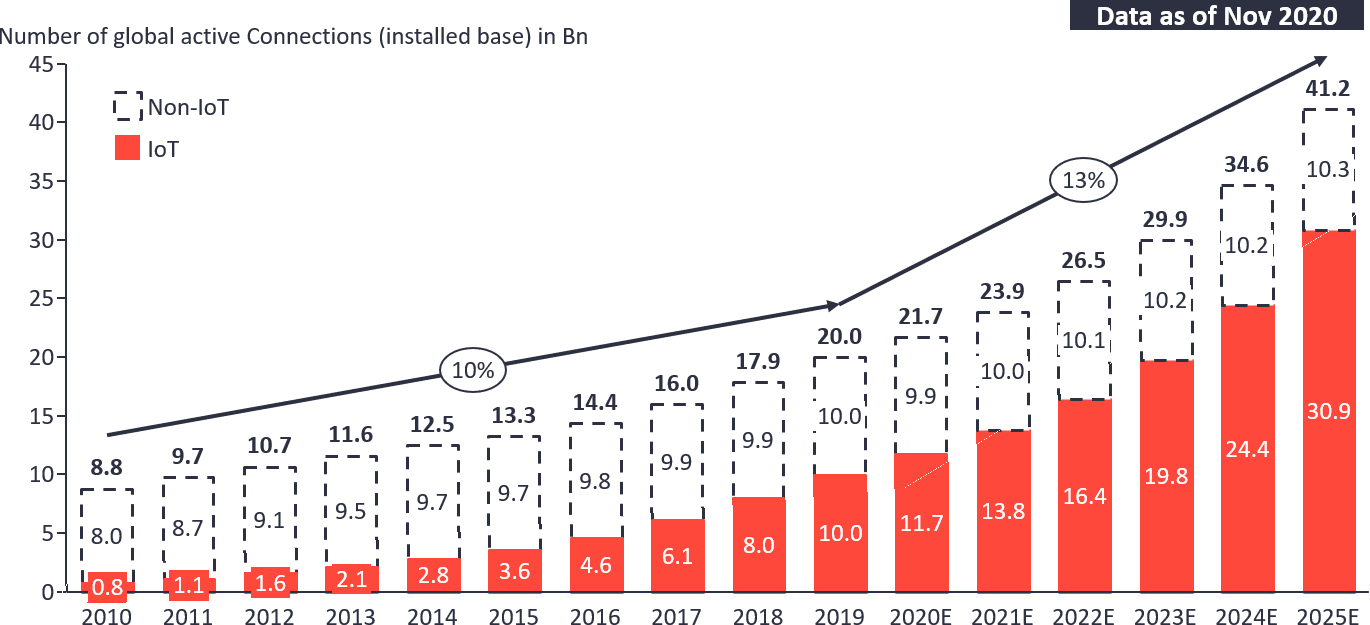
\includegraphics[width=0.9\linewidth]{IoT-connections-total-number-of-device-connections-min}
% 	\end{figure}
% 	\blfootnote{\tiny graphic by \url{iot-analytics.com}}
% \end{frame}
\begin{frame}
	\frametitle{Technology Trends}
	\begin{itemize}
        \item IoT is growing
		\item IoT is driving Big Data
		\item IoT is driving Semantic Web
		\item computing capabilities are increasing
		\begin{itemize}
         \item shifting computing and data storage to the edge
		 \item Cloud Computing $\rightarrow$ Fog Computing $\rightarrow$ Edge Computing
		\end{itemize}
	\end{itemize}
\end{frame}

\begin{frame}
	\frametitle{DBMS in Edge Computing}
    \begin{itemize}
        \item luposdate3000: Semantic Web DBMS adapted to IoT
        \item instances run on edge and fog devices
        \begin{itemize}
            \item multiplatform to support heterogeneity
            \item distribution of data storage and query processing
        \end{itemize}
    \end{itemize}
    \begin{itemize}
        \item current work
        \begin{itemize}
            \item simulator for integrating real DBMS into a modeled IoT environment
            \item protocol for distributed query processing
        \end{itemize}
    \end{itemize}
    \blfootnote{\tiny \url{https://github.com/luposdate3000/luposdate3000.git}}
\end{frame}
    
    
    
\begin{frame}
	\frametitle{Related Work}
    \begin{table}[htpb]
    \resizebox{\textwidth}{!}{
    \begin{tabular}{lp{1,4cm}p{3,3cm}p{1,4cm}p{1,7cm}p{1,4cm}p{1,7cm}p{1cm}p{1,3cm}p{1,9cm}}
    \hline
    \multirow{2}{*}{\emph{Simulator}} & \multicolumn{9}{l}{\emph{Features}}      \\ \cline{2-10} 
                            & Language 
                            & Purpose 
                            & Network Comm.
                            & Network Protocols 
                            & IoT Routing
                            & Node Performance 
                            & Real Data
                            & Energy 
                            & External Apps  
                            \\ \hline
    ns-3
    & C++, Python 
    & precise network simulation
    & $\checkmark\textsuperscript{\RNum{1}}$ 
    & $\checkmark\textsuperscript{\RNum{1}}$ 
    & $\checkmark\textsuperscript{\RNum{1}}$   
    &  
    & $\checkmark\textsuperscript{\RNum{1}}$ 
    & $\checkmark\textsuperscript{\RNum{1}}$  
    &  via file descriptor
    \\
    COOJA
    & Java, C 
    & precise WSN simulation in Contiki
    & $\checkmark$ 
    & $\checkmark$ 
    & $\checkmark$ 
    & $\checkmark$ 
    & $\checkmark\textsuperscript{\RNum{1}}$
    & $\checkmark$ 
    & 
    \\
    FogNetSim++
    & C++ 
    & apps in fog environments
    & $\checkmark$ 
    & $\checkmark$ 
    &  
    & $\checkmark$ 
    &  
    & $\checkmark$ 
    & 
    \\
    CloudSim
    & Java 
    & cloud computing
    & $\checkmark$
    &  
    &  
    & $\checkmark$ 
    &  
    & $\checkmark$
    & 
    \\
    IoTSim-Edge
    & Java 
    & app composition in edge computing
    & $\checkmark$
    & $\checkmark$
    &
    & $\checkmark$
    &
    & $\checkmark$
    &
    \\
    EdgeCloudSim
    & Java 
    & edge computing
    & $\checkmark$
    & 
    &
    & $\checkmark$
    &
    & $\checkmark$
    &
    \\
    IoTSim-Osmosis
    & Java 
    & app composition
    & $\checkmark$
    & $\checkmark$
    &
    & $\checkmark$
    &
    & $\checkmark$
    &
    \\
    iFogSim
    & Java 
    & fog computing with data streams
    & $\checkmark$
    & 
    &
    & $\checkmark$
    &
    & $\checkmark$
    &
    \\
    PureEdgeSim
    & Java 
    & edge computing
    & $\checkmark$
    & 
    &
    & $\checkmark$
    &
    & $\checkmark$
    &
    \\
    YAFS
    & Python 
    & dynamic infrastructures
    & $\checkmark$
    & 
    &
    & $\checkmark$
    &
    & $\checkmark$
    &
    \\
    MyiFogSim
    & Java 
    & mobile nodes
    & $\checkmark$
    & 
    &
    & $\checkmark$
    &
    & $\checkmark$
    &
    \\
    FogBed
    & Python 
    & real apps in containers
    & $\checkmark$
    & 
    &
    & $\checkmark$
    & $\checkmark$
    & 
    & via Docker
    \\
    (Proposed)
    & Kotlin
    & query processing with real DBMS
    & $\checkmark$
    & $\checkmark$
    & $\checkmark$
    & $\checkmark$
    & $\checkmark$
    &  
    & via Kotlin interface 
    \\
    \hline
    \end{tabular}}

\end{table}
\end{frame}

\section{Concept}

\begin{frame}
	\frametitle{IoT Environment}
	\begin{figure}
        \resizebox{0.8\linewidth}{!}{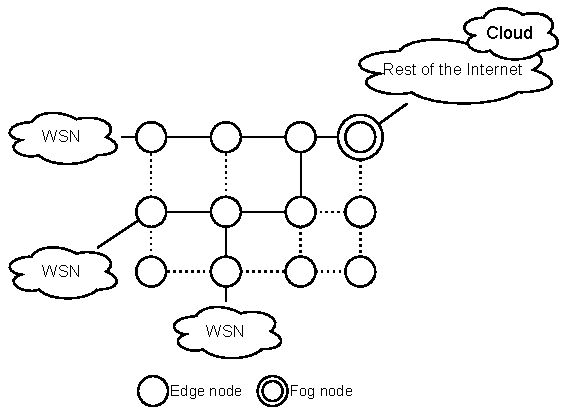
\includegraphics{edgemesh.pdf}}
		\centering
	\end{figure}
\end{frame}

\begin{frame}
	\frametitle{DBMS Instance Distribution}
    \begin{figure}
        \resizebox{0.8\linewidth}{!}{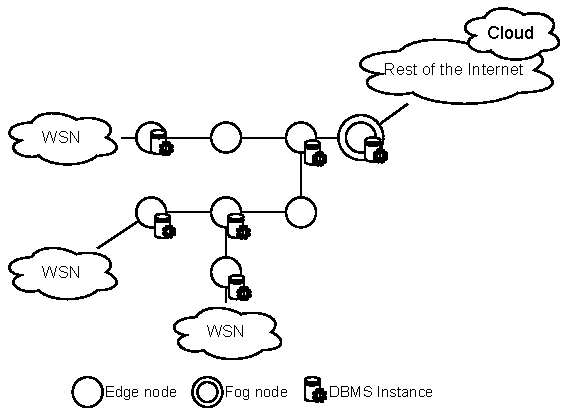
\includegraphics{edgemesh2.pdf}}
		\centering
	\end{figure}
\end{frame}
\begin{frame}
	\frametitle{Operator Graph Mapping}
    \begin{figure}
        \resizebox{0.8\linewidth}{!}{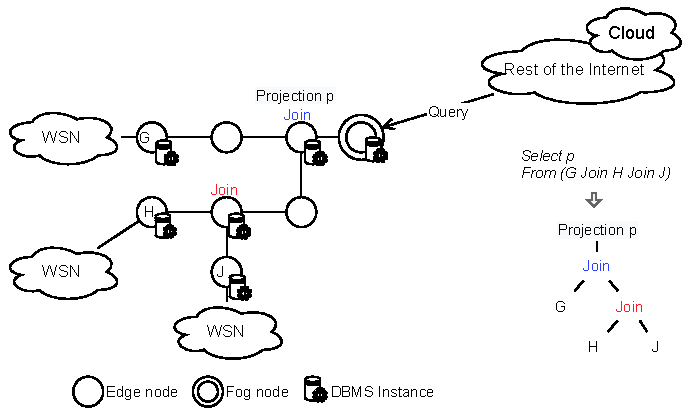
\includegraphics{figure_operatorgraph_mapping.pdf}}
		\centering
	\end{figure}
\end{frame}


\begin{frame}
	\frametitle{Query Processing Protocol}
    \begin{algorithmic}
        \Function{receive}{pck}
        \If{pck is QueryPackage}
            \State parse, send MulticastPackage
        \ElsIf{pck is MulticastPackage}
            \If{isLeafNode}
                \State  calculate, send ResultPackage or EndResultPackage
            \Else
                \State  prepare, send MulticastPackage
            \EndIf
        \ElsIf{pck is ResultPackage}
            \State calculate, send ResultPackage or EndResultPackage
        \EndIf
        \EndFunction
        
    \end{algorithmic}

    

\end{frame}

\begin{frame}
	\frametitle{Model: Parking Space Finder Application}
    \begin{figure}
        \resizebox{1.0\linewidth}{!}{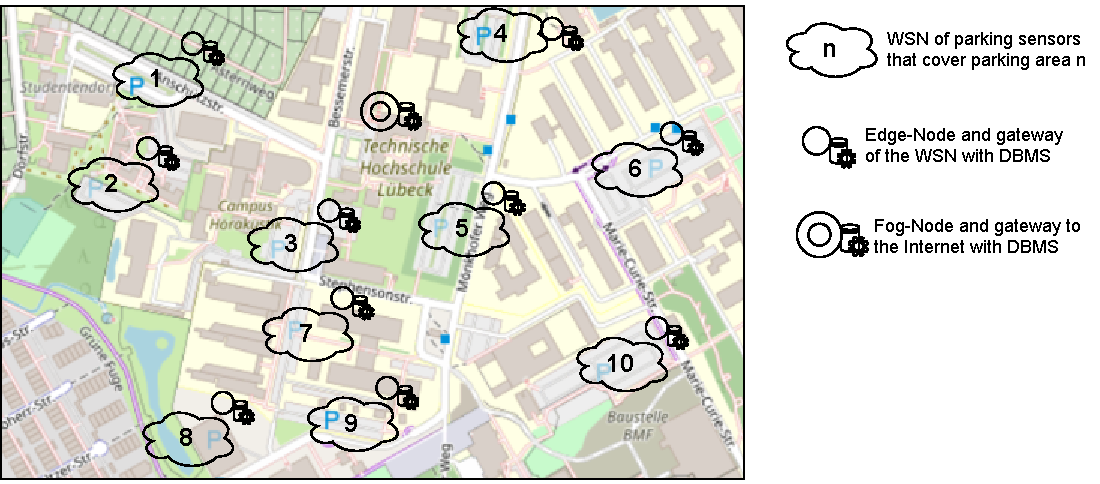
\includegraphics{figure_campus.pdf}}
        \centering
	\end{figure}
\end{frame}

\section{Evaluation}

\begin{frame}
	\frametitle{Protocol Evaluation}
    objective: less resource consumption than centralized processing \\
    $\rightarrow$ compare
    \medskip
    \begin{itemize}
        \item construct two topologies
        \begin{itemize}
         \item distributed case: 10 instances as data sinks for the WSNs + 1 instance as fog node
         \item centralized case: 1 instance as fog node and data sink for the WSNs
        \end{itemize}
        \medskip
        \item simulate
        \begin{itemize}
            \item insert sensor samples
            \item process 8 different SPARQL queries
        \end{itemize}
    \end{itemize}
\end{frame}


\begin{frame}
    \frametitle{Visualization}

    \begin{figure}
        \resizebox{0.65\linewidth}{!}{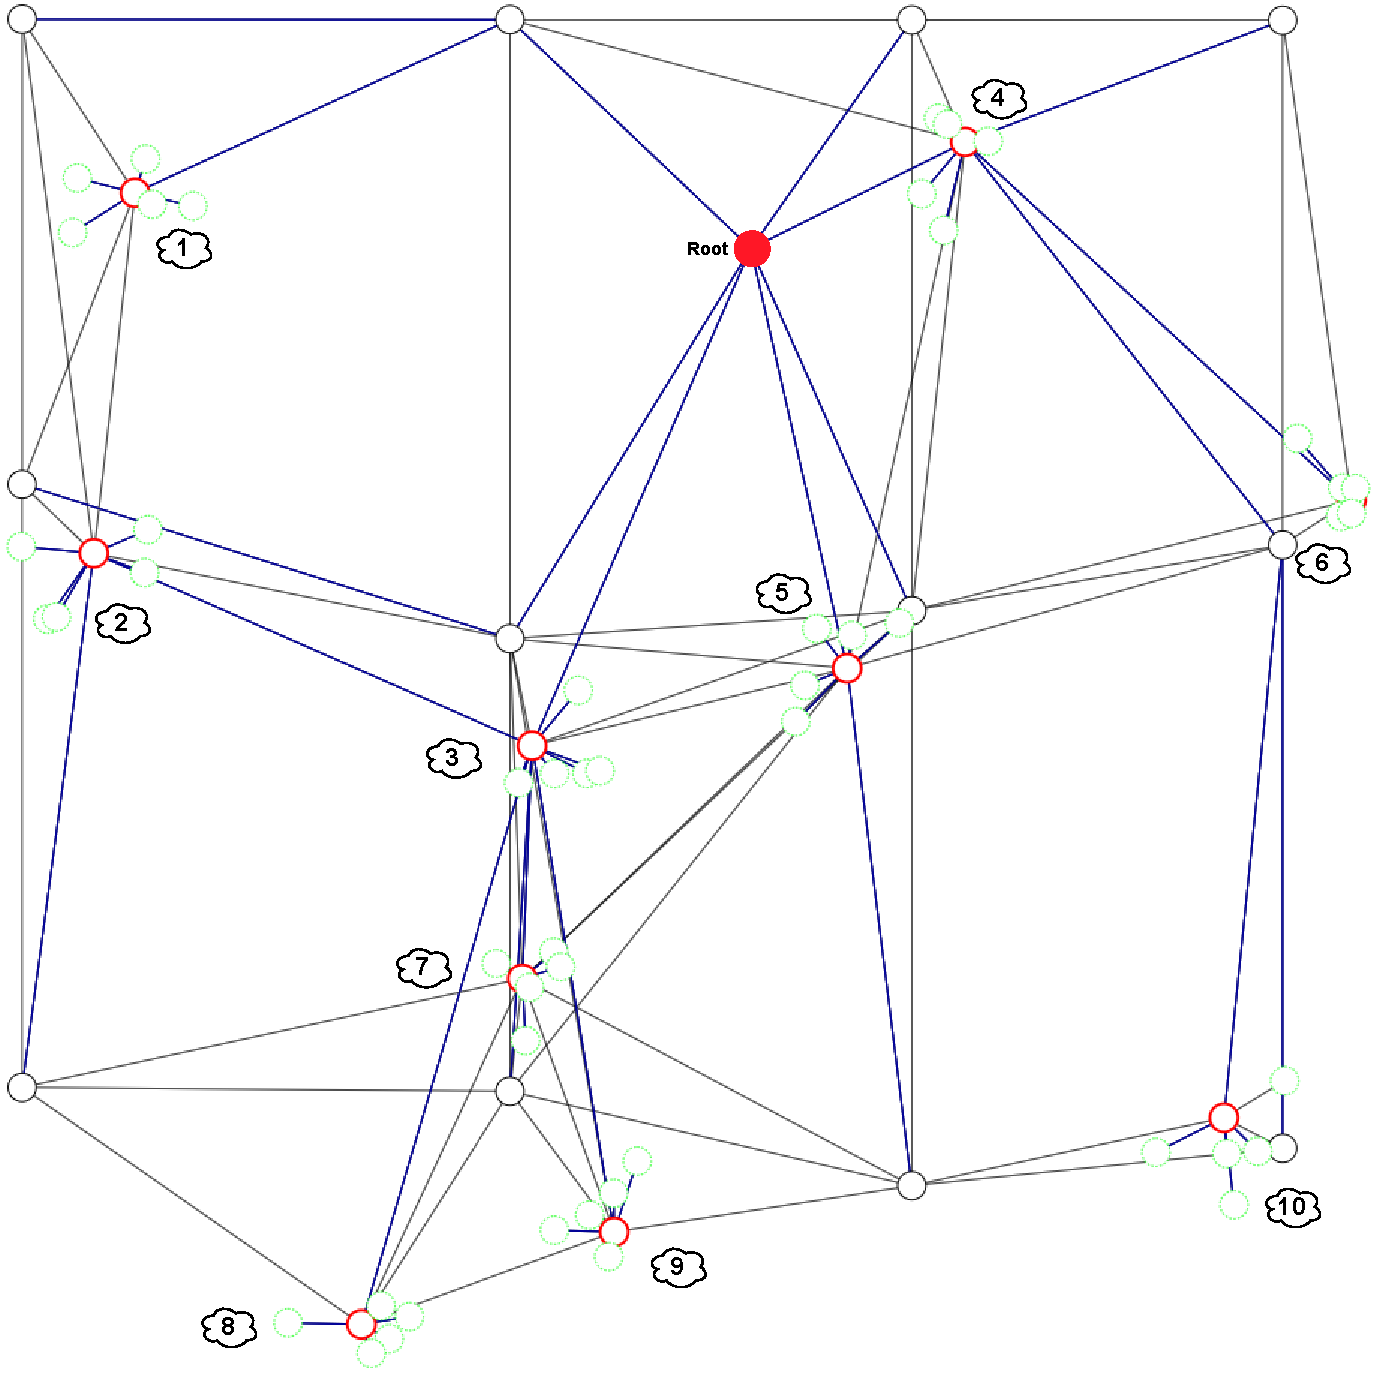
\includegraphics{figure_visualization.pdf}}
        \raggedleft
	\end{figure}
    \tikz [remember picture,overlay]
    \node at
    ([yshift=3cm,xshift=-4cm]current page.south) 
    %or: (current page.center)
    {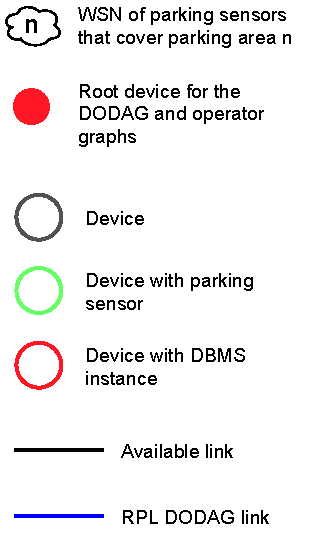
\includegraphics[width=0.2\textwidth]{figure_visualization_legend.pdf}};
\end{frame}

\begin{frame}
\frametitle{Simulation Results}
\begin{table}[htpb]

  \resizebox{0.9\textwidth}{!}{
    \begin{tabular}{c|cc|cc}
    \multicolumn{1}{c}{} & \multicolumn{2}{c}{Centralized Case} & \multicolumn{2}{c}{Distributed Case}\\
    & Sent Packages & Kilobytes Traffic & Sent Packages & Kilobytes Traffic
    \\ \hline
    Only Sample Inserts & 500 & 724 & 29060 & 9330\\[3ex]
    Q1 {\tiny Listing A.2} & 500 & 724 & 29080 & 9451\\[3ex]
    Q2 {\tiny Listing A.3} & 500 & 724 & 29080 & 9384\\[3ex]
    Q3 {\tiny Listing A.4} & 500 & 724 & 29132 & 9459\\[3ex]
    Q4 {\tiny Listing A.5} & 500 & 724 & 29080 & 9431\\[3ex]
    Q5 {\tiny Listing A.6} & 500 & 724 & 29118 & 9413\\[3ex]
    Q6 {\tiny Listing A.7} & 500 & 724 & 29216 & 9737\\[3ex]
    Q7 {\tiny Listing A.8} & 500 & 724 & 29216 & 9761\\[3ex]
    Q8 {\tiny Listing 3.5} & 500 & 724 & 29216 & 9726
    \end{tabular}}
\end{table}
\end{frame}


\begin{frame}
	\frametitle{Result Analysis}
    \begin{itemize}
        \item distributed case is worse due to the current sensor data distribution
        \begin{itemize}
            \item inserting a sample causes up to 66 messages
        \end{itemize}
        \item without sensor data distribution: could perform better than centralized case
    \end{itemize}
    
    
    \begin{table}[htpb]
    \resizebox{0.9\textwidth}{!}{
    \begin{tabular}{c|cc|cc}
    \multicolumn{1}{c}{} & \multicolumn{2}{c}{Centralized Case} & \multicolumn{2}{c}{Distributed Case (Dummy)}\\
    & Sent Packages & Kilobytes Traffic & Sent Packages & Kilobytes Traffic
    \\ \hline
    Only Sample Inserts & 500 & 724 & 500 & 258
    \end{tabular}}
\end{table}
        \begin{itemize}
        \item distributed query processing can have a maximum of $724 - 258 = 466$ kilobytes of traffic
        \item query processing traffic is always less than $466$ kilobytes!
    \end{itemize}
\end{frame}

\section{Conclusion}
\begin{frame}
	\frametitle{Summary and Future Work}
	\begin{itemize}
		\item summary
		\begin{itemize}
			\item new test environment for the development of IoT DBMS
			\item new protocol design for distributed query processing
		\end{itemize}
		\item future work
		\begin{itemize}
			\item optimize sensor data distribution
			\item optimize package sizes
			\item compare execution times
		\end{itemize}
	\end{itemize}
\end{frame}



\end{document} 
